% !TeX spellcheck = id_ID
% Tipe dokumen adalah report dengan satu kolom. 
% Menggatur setting halaman 
\documentclass[12pt, a4paper, onecolumn, oneside, final]{report}

% Load konfigurasi LaTeX untuk tipe laporan thesis
\usepackage{usd}
\usepackage{enumitem}
\usepackage{amsfonts}
\usepackage{listings}
\usepackage{subcaption}


\setlength{\parindent}{0.75cm}
\renewcommand{\arraystretch}{1.5}

% Daftar pemenggalan suku kata dan istilah dalam LaTeX
%
% Hyphenation untuk Indonesia 
%
% @author  Enggar Alfianto
% @version 1.00
% 
% Tambahkan cara pemenggalan kata-kata yang salah dipenggal secara otomatis 
% oleh LaTeX. Jika kata tersebut dapat dipenggal dengan benar, maka tidak 
% perlu ditambahkan dalam berkas ini. Tanda pemenggalan kata menggunakan 
% tanda '-'; contoh:
% menarik
%   --> pemenggalan: me-na-rik
%

\hyphenation{
    % alphabhet A
    a-na-li-sa a-tur 
    a-pli-ka-si 
    a-na-li-tik
    % alphabhet B
    ba-ngun-an 
    be-be-ra-pa 
    ber-ge-rak
    ber-ke-lan-jut-an 
    ber-pe-nga-ruh
    bim-bing-an 
    % alphabhet C
    ca-ri
    % alphabhet D
    di-sim-pan di-pim-pin de-ngan da-e-rah di-ba-ngun da-pat di-nya-ta-kan 
    di-sim-bol-kan di-pi-lih di-li-hat de-fi-ni-si
    di-rahmat-i
    di-identifi-kasi-kan
    di-re-pre-sen-ta-si-kan
    du-kung-an-nya
    % alphabhet E
    e-ner-gi eks-klu-sif
    % alphabhet F
    fa-si-li-tas
    fe-no-me-na
    % alphabhet G
    ga-bung-an ge-rak
    % alphabhet H
    ha-lang-an
    hamilton-nia-nya
    % alphabhet I
    % alphabhet J
    % alphabhet K
    ke-rapat-an
    ke-hi-lang-an
    ku-ning 
    kompu-tasi
    kua-li-tas ka-me-ra ke-mung-kin-an ke-se-pa-ham-an
    % alphabhet L
    ling-kung-an
    % alphabhet M
    me-nge-luar-kan
    me-neng-ah
    mem-perhitung-kan
    mem-ban-ding-kan
    meng-a-tas-i me-mung-kin-kan me-nge-na-i me-ngi-rim-kan 
    meng-u-bah meng-a-dap-ta-si me-nya-ta-kan mo-di-fi-ka-si
    meng-a-tur
    % alphabhet N
    nya-ta non-eks-klu-sif
    nano-tekno-logi
    % alphabhet O
    % alphabhet P
    pa-ling
	pe-nye-rap-an 
	pe-ngon-trol
    pe-mo-del-an
    pe-ran  pe-ran-an-nya
    pem-ba-ngun-an pre-si-den pe-me-rin-tah prio-ri-tas peng-am-bil-an 
    peng-ga-bung-an pe-nga-was-an pe-ngem-bang-an 
    pe-nga-ruh pa-ra-lel-is-me per-hi-tung-an per-ma-sa-lah-an 
    pen-ca-ri-an peng-struk-tur-an
    % alphabhet Q
    % alphabhet R
    ran-cang-an
    % alphabhet S
    si-mu-la-si sa-ngat
    se-bagai
    semi-konduktor
    % alphabhet T
    te-ngah
    ter-da-pat
    ter-selesai-kanya 
    % alphabhet U
    % alphabhet V
    % alphabhet W
    % alphabhet X
    % alphabhet Y
    % alphabhet Z
    % special
}

% Variabel baru untuk menyimpan nomor halaman
\newcounter{originalpagenumber}%

% Awal bagian penulisan laporan
\begin{document}

% Sampul Laporan
\begin{titlepage}
\begin{center}
\onehalfspacing\large\bfseries
\textsc{Penerapan Teknik Enkripsi Hill Cipher dalam Penyandian Citra}\\
\vspace{18pt}
\normalsize SKRIPSI \\
\vspace{12pt}
\linespread{1.5}\mdseries{	Diajukan untuk Memenuhi Salah Satu Syarat\\
Memperoleh Gelar Sarjana Komputer\\
Program Studi Teknik Informatika}
	\vspace{12pt}
	
	
\includegraphics[scale=0.4]{images/logo-usd.png}
	
	\vspace{12pt}
	DISUSUN OLEH: \\
	ENGELBERT ERIC SETIAWAN \\
	125314146
	
	\vspace{72pt}
	\textbf{
	 PROGRAM STUDI TEKNIK INFORMATIKA \\
	 JURUSAN TEKNIK INFORMATIKA\\
	FAKULTAS SAINS DAN TEKNOLOGI \\
	UNIVERSITAS SANATA DHARMA \\
	YOGYAKARTA\\
	2016
	}
	

	
\end{center}

\end{titlepage}

\newpage

% Daftar isi, gambar, dan tabel
% Gunakan penomeran Romawi (i, ii, iii, ...) setelah bagian ini.

\pagenumbering{roman}

% Judul Laporan
\begin{center}
	\onehalfspacing
	\large \bfseries PERANCANGAN SISTEM INFORMASI KOPERASI SIMPAN PINJAM BERBASIS WEB \\
	\vspace{1cm}
	 \large SKRIPSI \\
	 \normalsize Diajukan Untuk Melengkapi Salah Satu Syarat \\ Memperoleh Gelar Sarjana Komputer
	
	\vspace{2cm}
	
	
\includegraphics[width=6cm]{images/logo-unpam.png}
	
	\vspace{1cm}
	\large OLEH: \\
	IMRON ROSDIANA \\
	2010140419
	
	\vspace{3cm}
	
	\normalsize PROGRAM STUDI TEKNIK INFORMATIKA \\
	\large FAKULTAS TEKNIK \\
	UNIVERSITAS PAMULANG \\
	2014
	

	
\end{center}

\newpage

% Lembar Pernyataan
\phantomsection \addcontentsline{toc}{chapter}{LEMBAR PERNYATAAN}
%
% Lembar pengesahan Naskah

\chapter*{\uppercase{LEMBAR PERNYATAAN}}
\vspace{1cm}

\noindent Yang bertanda tangan di bawah ini:
\renewcommand{\arraystretch}{1.5}
\begin{table}[ht]
\begin{adjustwidth}{-0.15cm}{}
	\begin{tabular}{lll}
		Nama & : & Imron Rosdiadna \\
		NIM & : & 2010140419 \\
		Program Studi & : & Teknik Informatika \\
		Fakultas & : & Teknik \\
		Jenjang Pendidikan & : & Strata 1
	\end{tabular}
\end{adjustwidth}
\end{table} \\

\vspace{-1cm}
\noindent Menyatakan bahwa skripsi yang saya buat dengan judul:

\vspace{0.3cm}
\noindent PERANCANGAN SISTEM INFORMASI KOPERASI SIMPAN PINJAM BERBASIS WEB
\begin{enumerate}[nolistsep,leftmargin=0.5cm]
	\item Merupakan hasil karya tulis ilmiah sendiri, bukan merupakan karya yang pernah diajukan untuk memperoleh gelar akademik oleh pihak lain, dan bukan merupakan hasil plagiat.
	\item Saya ijinkan untuk dikelola oleh Universitas Pamulang sesuai dengan norma dan etika yang berlaku.
\end{enumerate}
Pernyataan ini saya buat dengan penuh tanggung jawab dan saya bersedia menerima konsekuensi apapun sesuai aturan yang berlaku apabila dikemudian hari pernyataan ini tidak benar.

\vspace{2cm}
\begin{table}[ht]
\begin{adjustwidth}{-0.15cm}{}
	\begin{tabular}{l}
	Pamulang, 01 Agustus 2014 \\[2cm]
	(Nama Orang)
	\end{tabular}
\end{adjustwidth}	
\end{table}

\newpage

% Lembar Persetujuan
\phantomsection \addcontentsline{toc}{chapter}{LEMBAR PERSETUJUAN}
%
% Lembar persetujuan
\doublespacing
\chapter*{\uppercase{LEMBAR PERSETUJUAN}}
\vspace{1cm}

\renewcommand{\arraystretch}{1.5}
\begin{table}[ht]
\begin{adjustwidth}{-0.15cm}{}
	\begin{tabularx}{\textwidth}{llX}
		Nama & : & Imron Rosdiadna \\
		NIM & : & 2010140419 \\
		Program Studi & : & Teknik Informatika \\
		Fakultas & : & Teknik \\
		Jenjang Pendidikan & : & Strata 1 \\
		Judul Skripsi & : & PERANCANGAN SISTEM INFORMASI KOPERASI SIMPAN PINJAM BERBASIS WEB
	\end{tabularx}
\end{adjustwidth}
\end{table}

\noindent Skripsi ini telah diperiksa dan disetujui. \\
Pamulang, 01 Agustus 2014

\vspace{3cm}
\begin{center}
\begin{minipage}{\linewidth}\centering
\underline{Pembimbing 1, S.Kom, M, Kom} \\
Pembimbing \\
\vspace{1cm}
Mengeetahui, \\
\vspace{3cm}
\underline{Kaprodi, S.Si, M.Si} \\
KaProdi Teknik Informatika
\end{minipage}
\end{center}

\newpage
\onehalfspacing

% Lembar Pengesahan
\phantomsection \addcontentsline{toc}{chapter}{LEMBAR PENGESAHAN}
%
% Lembar persetujuan
\doublespacing
\chapter*{\uppercase{LEMBAR PENGESAHAN}}

\renewcommand{\arraystretch}{1.5}
\begin{table}[ht]
\begin{adjustwidth}{-0.15cm}{}
	\begin{tabularx}{\textwidth}{llX}
		Nama & : & Imron Rosdiadna \\
		NIM & : & 2010140419 \\
		Program Studi & : & Teknik Informatika \\
		Fakultas & : & Teknik \\
		Jenjang Pendidikan & : & Strata 1 \\
		Judul Skripsi & : & PERANCANGAN SISTEM INFORMASI KOPERASI SIMPAN PINJAM BERBASIS WEB
	\end{tabularx}
\end{adjustwidth}
\end{table}

\onehalfspacing
\noindent Skripsi ini telah dipertahankan dihadapan dewan penguji ujian Skripsi Fakultas Teknik, Program Studi Teknik Informatika dan dinyatakan LULUS. \\
Pamulang, 01 Agustus 2014

\noindent
\vspace{0.3cm}
\begin{tabularx}{\linewidth}{XX}
\begin{minipage}{\linewidth}\centering
\vspace{2cm}
\underline{Penguji 1}\\
Penguji 1
\end{minipage} &
\begin{minipage}{\linewidth}\centering
\vspace{2cm}
\underline{Penguji 2}\\
Penguji 2
\end{minipage}
\end{tabularx}

\vspace{2.5cm}
\begin{center}
\begin{minipage}{\linewidth}\centering
\underline{Pembimbing, S.Kom, M, Kom} \\
Pembimbing \\
\vspace{1cm}
Mengeetahui, \\
\vspace{2.5cm}
\underline{Kaprodi, S.Si, M.Si} \\
KaProdi Teknik Informatika
\end{minipage}
\end{center}

\newpage
\onehalfspacing

% Lembar Abstract
\phantomsection \addcontentsline{toc}{chapter}{ABSTRACT}
%
% Halaman Abstract

\chapter*{ABSTRACT}

\begin{singlespace}
\blindtext \\[20pt]
Keywords: \textit{Information System, Testing Project}
\end{singlespace}

\newpage

% Lembar Abstrak
\phantomsection \addcontentsline{toc}{chapter}{ABSTRAK}
%
% Halaman Abstrak

\chapter*{ABSTRAK}

\begin{singlespace}
\blindtext \\[20pt]
Keywords: \textit{Sistem Informasi, Testing Project}
\end{singlespace}

\newpage

% Kata Pengantar
\phantomsection \addcontentsline{toc}{chapter}{KATA PENGANTAR}
% Kata Pengantar
\chapter*{KATA PENGANTAR}

\blindtext \\[2cm]

\hfill
\begin{minipage}[t]{4.9cm}
\centering
	Pamulang, 01 Agustus 2014 \\ [2cm]
	Imron Rosdiana
\end{minipage}

\newpage

\vspace*{-2.5cm}
\tableofcontents
\phantomsection
\addcontentsline{toc}{chapter}{DAFTAR ISI}
\clearpage
\vspace*{-2.5cm}
\listoftables
\phantomsection
\addcontentsline{toc}{chapter}{DAFTAR TABEL}
\clearpage
\vspace*{-2.5cm}
\listoffigures
\phantomsection
\addcontentsline{toc}{chapter}{DAFTAR GAMBAR}
\clearpage

% Gunakan penomeran Arab (1, 2, 3, ...) setelah bagian ini.
\pagenumbering{arabic}

%
% Atur header dan footer dalam dokumen.
% 
\renewcommand{\headrulewidth}{0.0pt}
	\fancyhf{} 
	\fancyhead[L]{} 
	\fancyhead[C]{} 
	\fancyhead[R]{\thepage} 
	\renewcommand{\headrulewidth}{0.0pt}
	\renewcommand{\footrulewidth}{0.0pt} 
\pagestyle{fancy}

\onehalfspacing
%-----------------------------------------------------------------------------%
\chapter{PENDAHULUAN}
%-----------------------------------------------------------------------------%

\vspace{6pt}

\section{Latar Belakang} \label{sec:latar_belakang}
Dekade ini, kita telah memasuki era informasi, yaitu era di mana informasi mengalir dengan arus yang sangat kencang dan hampir tak terbendung. Kemajuan teknologi telah memungkinkan kita untuk memanfaatkan arus informasi ini. Aplikasi multimedia terkini ditambah dengan kemampuan jaringan internet sekarang perlahan mengarahkan kita untuk bertukar informasi dengan gambar. Dengan adanya tren baru ini, diperlukan adanya mekanisme pengamanan tertentu agar informasi tidak jatuh ke tangan yang salah.

Untuk mengatasi efek negatif tersebut, ilmuwan komputer mengembangkan ilmu kriptografi, yaitu ilmu yang mempelajari prinsip dan metode untuk mengubah tulisan jelas (\textit{clear text}) menjadi tulisan yang tidak bermakna (\textit{cipher text}) dan kemudian dikembalikan lagi ke bentuk aslinya. Seiring dengan perkembangan zaman, kriptografi tidak melulu menyangkut teks, tapi dapat pula diaplikasikan ke jenis informasi lainnya, seperti citra, video, dan suara. Akan tetapi, perkembangan ini tidaklah tanpa biaya. Semakin rumit model informasi yang disandikan, semakin rumit pula algoritma penyandiannya.

Panighray dkk (2008) dalam penelitiannya mengembangkan metode enkripsi citra dengan metode Hill's Cipher yang termodifikasi. Metode ini menggunakan \emph{involutory key matrix}, yaitu matriks yang merupakan invers dirinya sendiri. Algoritma involutory key matrix ini diusulkan oleh Acharya dkk (2008) dalam jurnalnya yang berjudul “\textit{Novel Methods of Generating Self-Invertible Matrix for Hill Cipher Algorithm}”. Metode ini sudah cukup baik untuk menyandikan citra, akan tetapi matriks kuncinya dibuat secara acak. Penulis berusaha mengembangkan metode ini sehingga pengguna dapat menentukan sendiri matriks kuncinya.

Bertolak dari permasalahan di atas, penulis mengusulkan untuk membuat metode enkripsi yang berdasar dari penelitian Panighray dkk. dengan sedikit perubahan, yaitu menggunakan matriks kunci yang ditentukan oleh pengguna sendiri.
%\lipsum[4-5]

\section{Rumusan Masalah}
Berdasarkan latar belakang di atas dapat diidentifikasi masalah-masalah sebagai berikut:
\begin{enumerate}[nolistsep,leftmargin=1cm]
\item Bagaimanakah algoritma penyandian baru yang didasarkan metode Advanced Hill Cipher?
\item Bagaimana kehandalan metode yang diusulkan penulis dibandingkan dengan metode Hill Cipher yang asli?
\item Apakah metode yang diusulkan penulis layak untuk diterapkan untuk penyandian citra? Bagaimana pengujiannya?
\end{enumerate}

\section{Tujuan Penelitian}
\begin{enumerate}[nolistsep,leftmargin=1cm]
\item Menemukan metode penyandian baru berdasar metode Advanced Hill Cipher usulan Panighray dkk.
\item Menguji kehandalan metode yang diusulkan penulis.
\end{enumerate}

\section{Batasan Masalah}
Dalam penelitian ini, peneliti akan membatasi masalah yang akan diteliti antara lain:
\begin{enumerate}[nolistsep,leftmargin=1cm]
\item Citra yang dienkripsi berupa citra berwarna tiga kanal (\textit{RGB}) atau citra keabuan (\textit{grayscale}).
\item Format citra yang diolah adalah PNG, JPG, atau BMP.
\end{enumerate}

\section{Manfaat Penelitian}


\section{Metodologi Penelitian}
\subsection{Studi Literatur}
Studi literatur dilakukan untuk mendapatkan informasi terkait penelitian yang
dilakukan. Studi literatur dilakukan dengan cara mempelajari buku referensi, artikel
dan jurnal yang berkaitan dengan kriptografi dan pemrosesan citra.

\subsection{Percancangan Sistem}
Pada tahap ini dilakukan perancangan pembuatan sistem berdasarkan teori-teori yang didapatkan 
dari tahap sebelumnya.

\subsection{Pengumpulan Data}
Pada tahap ini dilakukan pengumpulan data yang digunakan untuk penelitian.

\subsection{Implementasi Sistem}
Tahap ini merupakan tahap di mana sistem diwujudkan. Sistem dibuat sesuai dengan rancangan 
pada tahap sebelumnya.

\subsection{Pengujian}
Setelah sistem selesai dibuat, data yang sudah terkumpul diuji menggunakan sistem tersebut
untuk kemudian diuji kesahihannya dibandingkan dengan teori yang ada.

\section{Sistematika Penulisan}
\subsection*{BAB I: PENDAHULUAN} %\textbf{BAB I: PENDAHULUAN}
\begin{addmargin}[0.75cm]{0em}
Bab ini berisi tentang latar belakang masalah, rumusan masalah, tujuan penelitian, batasan masalah, manfaat penelitian, metodologi penelitian, dan sistematika penulisan.
\end{addmargin}
\subsection*{BAB II: LANDASAN TEORI}
\begin{addmargin}[0.75cm]{0em}
Bab ini berisi tentang teori-teori yang mendukung atau berhubungan denga aplikasi ini.
\end{addmargin}
\subsection*{BAB III: ANALISA DAN PERANCANGAN SISTEM}
\begin{addmargin}[0.75cm]{0em}
Bab ini menjelaskan tentang proses menganalisa dan merancang sistem aplikasi ini.
\end{addmargin}
\subsection*{BAB IV: IMPLEMENTASI DAN PENGUJIAN}
\begin{addmargin}[0.75cm]{0em}
Bab ini berisi tentang implementasi dan pengujian sistem aplikasi yang telah dibuat.
\end{addmargin}
\subsection*{BAB V: KESIMPULAN DAN SARAN}
\begin{addmargin}[0.75cm]{0em}
Bab ini berisi tentang kesimpulan dan saran untuk mendukung perbaikan sistem aplikasi ini.
\end{addmargin}

\newpage
%-----------------------------------------------------------------------------%
\chapter{LANDASAN TEORI}
%-----------------------------------------------------------------------------%

%
\vspace{12pt}


\section{Kriptografi}
Kriptografi adalah ilmu yang melindungi data dan komunikasi. Objektif utama
kriptografi adalah untuk memungkinkan dua pihak berkomunikasi lewat saluran
tidak aman sedemikian rupa sehingga pihak ketiga tidak dapat memahami apa yang
sedang dibicarakan.\par
Salah satu komponen utamanya melibatkan pertukaran pesan atau informasi antara
dua pihak dengan mengubah wujud pesan/data dengan berbagai cara yang bertujuan
untuk membuat pihak lain kesulitan "menguping" pembicaraan. Aspek lainnya
termasuk otentikasi -- proses meyakinkan penerima pesan bahwa pesan benar-benar
berasal dari sumber yang asli (bukan dari pengirim lain yang menyamar) -- dan
integritas -- bahwa pesan yang sampai ke penerima adalah benar pesan yang
dikirim oleh pengirim tanpa mengalami perubahan sedikitpun.
\section{Matriks}
Matriks merupakan struktur data yang sangat umum dan natural dalam komputasi,
terdiri atas kumpulan angka yang membentuk persegi panjang. Matriks memiliki
beberapa karakteristik penting, yaitu:
\begin{enumerate}[label=\alph*.]
\item Dimensi\\Sebuah matriks dengan $n$ baris dan $m$ kolom disebut sebagai matriks $n\times m$.
Dua bilangan inilah yang disebut sebagai dimensi sebuah matriks. Jika $n = m$, maka
matriks dikatakan sebagai matriks persegi.
\item Elemen\\Setiap angka dalam sebuah matriks merupakan sebuah elemen. Sebuah
elemen $a_{ij}$ dari matriks $A$ terletak pada baris $i$ dan kolom $j$.
\item Vektor\\Dalam hubungannya dengan matriks, sebuah vektor $v$ adalah sebuah
matriks yang berdimensi $1\times n$ atau $n\times 1$.
\[
\begin{bmatrix}
  a_{11} & a_{12} & a_{13} & \cdots & a_{1m} \\
  a_{21} & a_{22} & a_{23} & \cdots & a_{2m} \\
  a_{31} & a_{32} & a_{33} & \cdots & a_{3m} \\
  \vdots  & \vdots  & \vdots & \ddots & \vdots  \\
  a_{n1} & a_{n2} & a_{n3} & \cdots & a_{nm} 
 \end{bmatrix}
 \]
\end{enumerate}

\subsection{Operasi Matriks}
Layaknya angka, matriks pun memiliki beberapa operasi aritmatika. Beberapa
operasi matriks sangat trivial, sisanya memerlukan penge-tahuan khusus. Dalam
penelitian ini, penulis akan menggunakan beberapa operasi matriks dasar, yaitu:

\begin{enumerate}[label=\alph*.]

\item Penjumlahan dan pengurangan matriks\\Penjumlahan dan pengurangan matriks
merupakan salah satu operasi trivial. Operasi penjumlahan dan pengurangan
matriks dilakukan elemen per elemen. Syarat penjumlahan dan pengurangan matriks
adalah kedua matriks harus memiliki dimensi yang sama.
\begin{equation} \label{penjumlahan_matriks}
[a_{ij}] \pm [b_{ij}] = [a_{ij}\pm b_{ij}] \text{, untuk setiap }  i \text{ dan } j
\end{equation}

\item Perkalian skalar\\Perkalian skalar juga merupakan operasi trivial. Jika k adalah sebuah
konstanta, maka kA adalah perkalian skalar matriks A dengan k,
didefinisikan sebagai matriks dengan elemen-elemen a ij yang
dikalikan dengan k.
\begin{equation}
k[a_{ij}] = [ka_{ij}] \text{, untuk setiap } i \text{ dan }j
\end{equation} 

\item Perkalian matriks\\Jika A adalah matriks $n \times m$ dan B adalah matriks $m \times r$ maka
perkalian matrix $C = A \times B$ didefinisikan sebagai
\begin{equation}
	c_{ij}=\sum_{k=1}^m{a_{ik}b_{kj}}\text{ , } \left(
	\begin{array}{l}
		i=1, 2, 3, \dotsc, n\\
		j=1, 2, 3, \dotsc, m
	\end{array}\right)
\end{equation} 
Matriks $C$ hasil perkalian akan berdimensi $n\times r$.

\subsection{Matriks identitas}
Untuk sebuah bilangan bulat positif $n$, matriks identitas $n \times{n}$,
dinotasikan sebagai $I_n$ atau $I$ saja, adalah matriks 
\begin{equation}
	\left[\delta_{ij}\right]=
	\begin{cases}
		1& \text{jika $i=j$}\\
		0& \text{jika $i \neq j$}
	\end{cases}
\end{equation}
Penamaan ini didasarkan pada sifatnya yang mirip dengan angka 1
sebagai identitas perkalian pada bilangan real: perkalian sebarang
matriks persegi $A$ dengan $I$ menghasilkan $A$.

\subsection{Invers matriks}
Sebuah matriks persegi A dinyatakan \textit{invertible} (memiliki invers) jika dan
hanya jika ada matriks lain $A^{-1}$ yang memenuhi persamaan berikut:
\begin{equation}
	AA^{-1}=A^{-1}A=I
\end{equation}
\end{enumerate}

\section{Operasi bilangan bulat modular}
Bilangan mod(ulus) $m$, $\mathbb{Z}_m$ , adalah himpunan $\lbrace x|x = 0, 1, 2, 3, \dotsc , m - 2, m -
1 \rbrace $. Operasi yang berlaku di domain bilangan bulat berlaku juga di bilangan bulat
mod m. Secara umum, operasi modulus m didefinisikan secara rekursif sebagai
berikut:
\begin{equation}
c \bmod{m}= \begin{cases}
	(m-c)\bmod{m}	&\text{jika }c<0\\
	c				&\text{jika }0\leq c<m\\
	(c-m)\bmod{m}	&\text{jika }c\geq m
\end{cases}
\end{equation}

\subsection{Penjumlahan dan pengurangan}
Penjumlahan dan pengurangan bilangan bulat modulus $m$ didefinisikan sebagai berikut:
\begin{equation}
\begin{array}{lrcl}
	\text{jika}	& a\pm{b}			&=&c\\
	\text{maka}	& (a\pm b)\bmod m	&=&c\bmod m\\
	\;			&\;					&=&(a\bmod m)\pm (b\bmod m)
\end{array}
\end{equation}

\subsection{Perkalian}\
\begin{equation}
	\begin{array}{lrcl}
		\text{jika}	& a\times b			&=&c\\
		\text{maka}	& (a\times b)\bmod m&=&c\bmod m\\
		\;			&\;					&=&(a\bmod m)\times (b\bmod m)\\
	\end{array}
\end{equation}

\subsection{Pembagian (sebagai invers perkalian)}
$a\div b\bmod m=c$ jika dan hanya jika ada $c\in \mathbb{Z}_m$ yang memenuhi persamaan 
$(b\times c)\bmod m=a$.

\subsection{\textit{Multiplicative inverse}}
Invers dari $b$, $b^{-1}$ adalah sebuah bilangan $c\bmod m$ yang memenuhi 
persamaan $(b\times c)\bmod m=1$.\par
Sebuah bilangan $c\bmod m$ memiliki inverse jika $c$ relatif prima (\textit{coprime})
terhadap $m$, yaitu $\operatorname{gcd}(c,m)=1$. Oleh karena itu, penting untuk memilih 
modulo yang benar sehingga sebagian besar $c\in\mathbb{Z}_m$ memiliki invers.

\section{Matriks Modular}
Matriks modular adalah matriks dengan elemen-elemen bilangan modulus.
Matriks modular memiliki aturan-aturan yang hampir sama dengan matriks real
tetapi pada domain yang berbeda, yaitu bilangan modulus. Operasi-operasinya
pun didasarkan pada operasi modulus.
\newpage
%-----------------------------------------------------------------------------%
\chapter{ANALISA DAN PERANCANGAN SISTEM}
%-----------------------------------------------------------------------------%

%
\vspace{4.5pt}

\section{Analisa Sistem}

\subsection{Analisa Sistem Saat Ini}
Analisa sistem pendukung keputusan dalam penentuan penjurusan dibuat oleh peneliti dalam bentuk use case diagram yang mewakili secara sederhana dan bisa dijadikan sebagai bahan dalam evaluasi sistem yang berjalan, sehingga sistem dapat terlihat tanpa harus mengetahui secara detail prosedur yang berjalan.
\begin{figure}[ht]
	\centering
	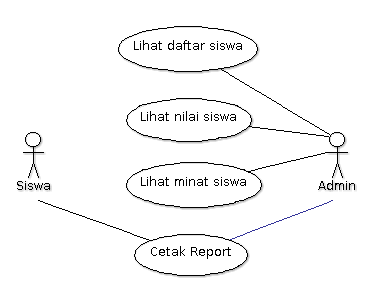
\includegraphics[width=10cm]{images/UseCaseDiagramSistemSaatIni}
	\caption{Use Case Diagram Analisa Sistem Saat Ini}
\end{figure}

\newpage
\noindent Dibawah ini merupakan deskripsi dari use case yang sedang berjalan:
\begin{enumerate}[nolistsep,leftmargin=0.5cm]
\item \textit{Admin} melihat daftar siswa.
\item \textit{Admin} melihat nilai setiap siswa.
\item \textit{Admin} melihat minat setiap siswa.
\item \textit{Admin} mencetak hasil keputusan.
\item Siswa melihat laporan penjurusan yang telah dicetak oleh \textit{admin}
\end{enumerate}

\subsection{Evaluasi Sistem Saat Ini}

\begin{table}[ht]
\centering
\caption{Permasalahan dan Solusinya}
\begin{tabular}{|>{\raggedright}p{5cm}|p{2.5cm}|>{\raggedright}p{5cm}|}
 \hline
 \multicolumn{1}{|c}{\bfseries Masalah} & \multicolumn{1}{|c|}{\bfseries Aktor} & \multicolumn{1}{c|}{\bfseries Solusi} \\ 
  \hline
\begin{enumerate}
   	\item Masalah masalah masalah Masalah masalah masalah Masalah masalah masalah Masalah masalah masalah.
   	\item Masalah masalah masalah Masalah masalah masalah Masalah masalah masalah Masalah masalah masalah.
   	\item Masalah masalah masalah Masalah masalah masalah Masalah masalah masalah Masalah masalah masalah.
   \end{enumerate} &
   \begin{enumerate}
  	\item Aktor 1
  	\item Aktor 2
  \end{enumerate} &
  \begin{enumerate}
  \item Solusi solusi solusi Solusi solusi solusi Solusi solusi solusi Solusi solusi solusi Solusi solusi solusi.
  \item Solusi solusi solusi Solusi solusi solusi Solusi solusi solusi Solusi solusi solusi Solusi solusi solusi.
  \item Solusi solusi solusi Solusi solusi solusi Solusi solusi solusi Solusi solusi solusi Solusi solusi solusi.
  \end{enumerate}
     \tabularnewline
  \hline
 \end{tabular}
\end{table}

\subsection{Model yang Diusulkan}

\subsection{Acitivity Diagram yang Diusulkan}

\subsection{Perancangan Prosedur Sistem}

\subsubsection{Use Case Diagram}

\subsubsection{Activity Diagram}
\begin{enumerate}[nolistsep,leftmargin=0.5cm]
\item \textit{Activity diagram} satu

\begin{enumerate}[label=\alph*.]
	\item Item 1.
	\item Item 2.
	\end{enumerate}
\item Dua
\end{enumerate}

\subsubsection{Class Diagram}

\subsubsection{Sequence Diagram}

\subsection{Perancangan Antarmuka (Interface)}

\newpage
%-----------------------------------------------------------------------------%
\chapter{IMPLEMENTASI DAN PENGUJIAN}
%-----------------------------------------------------------------------------%

%
\vspace{4.5pt}

\section{Implementasi}

\subsection{Lingkungan Perangkat Lunak}

\subsection{Spesifikasi Perangkat Keras}

\subsection{Impelementasi Antarmuka}

\subsubsection{Impelementasi Halaman Utama}

\subsubsection{Implementasi Menu File}

\subsubsection{Implementasi Menu}

\subsection{Pengguna Program}

\section{Pengujian}

\subsection{Pengujian Blackbox}

\subsection{Pengujian Whitebox}

\newpage
%-----------------------------------------------------------------------------%
\chapter{PENUTUP}
%-----------------------------------------------------------------------------%

%
\vspace{12pt}

\section{Kesimpulan}
Secara umum, algoritma Hill Cipher cukup baik untuk digunakan sebagai metode enkripsi citra.
Karena sifat dasarnya sebagai linear kombinator, Hill Cipher mampu menyebarkan informasi
(dalam hal ini, intensitas warna) sehingga cukup resisten terhadap \emph{statistical attack}.
Akan tetapi, karena sifat linearitasnya itu juga, Hill Cipher menjadi lemah terhadap \emph{known-
plaintext attack}. Akan tetapi kelemahan ini bisa dikurangi dengan menambah panjang kunci; semakin 
panjang kuncinya, akan semakin sulit melakukan \emph{known-plaintext attack}. Namun demikian, pertambahan
panjang kunci berimbas pada makin lamanya proses enkripsi (sekaligus dekripsi) dan pembuatan invers 
matriks kunci.

\section{Saran}
Penelitian ini tidak mencakup aspek transmisi dari citra terenkripsi, sehingga pada prakteknya dapat
terjadi adanya \emph{transmission error} yang berakibat citra yang diterima tidak sama dengan citra 
yang ditransmisikan. Selain itu tidak menutup kemungkinan juga bahwa pengguna lupa sebagian atau 
bahkan seluruh kunci yang berakibat pada citra yang tidak bisa terdekripsi dengan baik (atau malah 
tidak dapat terdekripsi sama sekali). Oleh karena itu beberapa hal yang menjadi saran untuk penelitian
selanjutnya:
\begin{itemize}
\item Bagaimana cara transmisi \emph{cipherimage} sehingga tidak ada \emph{information loss}.
\item Bagaimana cara memperbaiki \emph{cipherimage} yang korup sehingga masih dapat didekripsi sebagian.
\item Bagaimana cara memperbaiki kunci yang dilupakan sebagian sehingga masih ada informasi yang bisa didapat dari proses dekripsi.
\item Bagaimana cara penyimpanan dan distribusi kunci sehingga hanya orang yang berhak yang dapat memilikinya.
\end{itemize}
Selain itu, untuk khalayak umum penulis memberi saran:
\begin{itemize}
\item Jangan mengirim informasi sensitif melalui jalur tidak aman. Sekuat apapun algoritma enkripsi tidak
akan mampu mengkompensasi kerugian yang timbul atas kecerobohan manusia.
\item Ketika menyangkut informasi sensitif, jangan percaya siapapun.
\item Pertimbangkan juga untuk menggunakan steganografi yang dikombinasikan dengan kriptografi untuk
mengurangi ketertarikan pihak ketiga.
\end{itemize}

\newpage

% Merubah Nama Bibliografi ke Daftar Pustaka
\renewcommand{\bibname}{DAFTAR PUSTAKA}
\phantomsection
\addcontentsline{toc}{chapter}{DAFTAR PUSTAKA}
% Daftar Pustaka
%
% Daftar Pustaka 
% 
%Format Penulisan Daftar Pustaka yang di Sesuai dengan aturan penulisan Unair
%==========================================================================================
%\bibitem[Nama,tahun]{citasi}
%Nama Pengarang, Tahun,
%\newblock \emph{Judul dan keterangan}.
%\newblock Penerbit, Kota.
%========================================================================================== 
% Tambahkan pustaka yang digunakan setelah perintah berikut. 
% 
\begin{thebibliography}{7}
%\bibliographystyle{unsrt}
\providecommand{\natexlab}[1]{#1}
\providecommand{\url}[1]{\texttt{#1}}
\expandafter\ifx\csname urlstyle\endcsname\relax
  \providecommand{\doi}[1]{doi: #1}\else
  \providecommand{\doi}{doi: \begingroup \urlstyle{rm}\Url}\fi

\bibitem[Akbar,2008]{taufik}
Akbar, T, 2008,
\newblock \emph{Penentuan Spektrum Aksi \textit{Porphyrin} Dengan Metode
  Semi-Empirik \textit{Hartree-Fock} (Skripsi)}.
\newblock Departemen Fisika, Universitas Airlangga.

\bibitem[Arias,2005]{arias}
Arias.T.A, 2005,
\newblock Notes on the ab initio theory of molecules and solids: Density
  functional theory (dft).
\newblock Cornell University.

\bibitem[Darmawan,2009]{darmawan}
Darmawan, E, 2009,
\newblock \emph{Pemrograman Dasar C-Java-C\#}.
\newblock Penerbit Informatika, Bandung.

\bibitem[Haken,1994]{haken}
Haken, Hermann. W.C, 1994,
\newblock \emph{{M}olecular {P}hysics and {E}lements of {Q}uantum {C}hemistry}.
\newblock Springer. USA

\bibitem[Hiroshi,2009]{hiroshi}
Hiroshi Katayama-Yoshida, 2009,
\newblock Computational Nano-Materials Design for Spinodal Nanotechnology.
\newblock Osaka University Japan

\bibitem[Rinaldi,2008]{munir}
Rinaldi. M, 2008,
\newblock \emph{Metode Numerik}.
\newblock Penerbit Informatika, Bandung

\bibitem[Siregar,2010]{rustam}
Siregar. R.E, 2010,
\newblock \emph{Teori dan Aplikasi Fisika Kuantum}.
\newblock Widya Padjadjaran, Bandung.

\bibitem[S.S.~David,2009]{david}
Shols.~David,S .A.~J, 2009,
\newblock \emph{{D}ENSITY {F}UNCTIONAL {T}HEORY A {P}ractical {I}ntroduction}.
\newblock John Wiley and Sons, Inc,

\bibitem[William H.~Press,1999]{william}
S.~A.~T. William H.~Press, Brian P.~Flannery, 1999, 
\newblock \emph{{N}umerical {R}ecipes in {C}. {T}he {A}rt of {S}cientific
  {C}omputing}.
\newblock Cambridge University Press.


\bibitem[NIST(2011)]{nist}
http://physics.nist.gov/PhysRefData/DFTdata.
\newblock Atomic Reference Data for Electron Structure Calculation.
\newblock 08 Februari 2011.


\end{thebibliography}



%
% Lampiran 
%

\setcounter{originalpagenumber}{\number\value{page}}%
\setcounter{page}{0}
\pagenumbering{arabic}

\onehalfspacing
\begin{appendix}
	%
% @author  Andreas Febrian
% @version 1.00 
% 
% Hanya sebuah pembatas bertuliskan LAMPIRAN ditengah halaman. 
% 

\begin{titlepage}
	\centering 
	\vspace*{6cm}
	\noindent \Huge{LAMPIRAN}
\end{titlepage}
\end{appendix}

\pagenumbering{arabic}% 
\setcounter{page}{\number\value{originalpagenumber}}
\clearpage
\phantomsection \addcontentsline{toc}{chapter}{LAMPIRAN}

%-----------------------------------------------------------------------------%
\section*{Coding Login Aplikasi}
%-----------------------------------------------------------------------------%



\end{document}